\subsubsection{KP05. Manajemen Voucher}
\label{kp05}

	\begin{figure}[H]
		\centering
		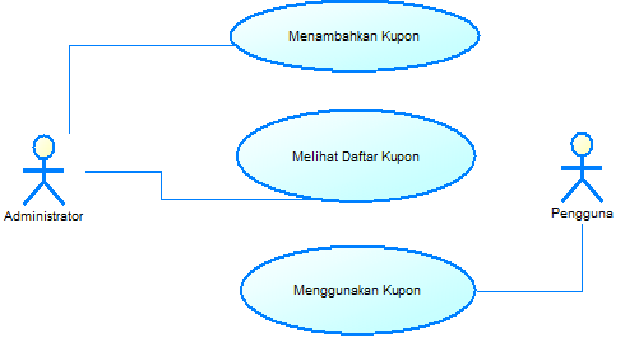
\includegraphics
		[width=\textwidth]{images/bab3/usecasediagram/ucd-06.png}
		\caption{Diagram Kasus Penggunaan Manajemen Kupon}
		\label{ucd.06}
	\end{figure}
	Kasus penggunaan ini seluruhnya digunakan oleh \textit{administrator} aplikasi dan dilakukan di sistem terpisah. Kasus penggunaan ditujukan untuk mempermudah \textit{administrator} dalam memanajemen kupon yang dibagikan oleh pengguna.

	% Menambahkan voucher
		% Memasukkan kupon
	
	\begin{table}[H]
		\centering
		\begin{tabular}{|r|p{8cm}|}
			\hline
			\textbf{Kode}
			& UC-05.01
			\\ \hline
			\textbf{Nama}
			& \textbf{Menambahkan Kupon} 
			\\ \hline
			\textbf{Aktor}    
			& Administrator 
			\\ \hline
			\textbf{Deskripsi}
			& Administrator ingin menggunakan kupon/voucher yang ia miliki untuk pada sebuah transaksi
			\\ \hline
			\textbf{Tipe}
			& Fungsional 
			\\ \hline
			\textbf{\textit{Precondition}}
			& Kupon baru belum berhasil tersimpan di sistem
			\\ \hline
			\textbf{\textit{Postcondition}} 
			& Kupon baru berhasil tersimpan di sistem
			\\ \hline
			\multicolumn{2}{|c|}
			{\textbf{Alur Kejadian Normal}}
			\\ \hline
			\multicolumn{1}{|l|}{} & 
			\begin{enumerate}
				\item Administrator membuka halaman 'Tambah Kupon'
				\item Sistem menampilkan halaman form Tambah Kupon
				\item Administrator memasukkan informasi kupon baru yang akan ditambahkan
				\item Sistem mengecek permintaan penggunaan kupon,jika permintaan dapat diverifikasi dan valid, sistem me\textit{redirect} ke halaman manajemen kupon.
				% \item \label{uc0301-show1page}Sistem menampilkan halaman yang berisi form pendaftaran barang
				% \item \label{al-0301-a} Sistem memvalidasi data yang dimasukkan pengguna
			\end{enumerate}
			\\ \hline
			\multicolumn{2}{|c|}{\textbf{Alur Kejadian Alternatif}} \\ \hline
			\multicolumn{1}{|l|}{}                   
			& -
			\\ \hline
		\end{tabular}
		\caption{Spesifikasi Kasus Penggunaan : Menambahkan Kupon}
		\label{uc06.01}
	\end{table}
	
	% Melihat daftar voucher
		% Memasukkan kupon
	
	\begin{table}[H]
		\centering
		\begin{tabular}{|r|p{8cm}|}
			\hline
			\textbf{Kode}
			& UC-05.02
			\\ \hline
			\textbf{Nama}
			& \textbf{Memasukkan Kupon pada Transaksi} 
			\\ \hline
			\textbf{Aktor}    
			& Pengguna 
			\\ \hline
			\textbf{Deskripsi}
			& Pengguna ingin menggunakan kupon/voucher yang ia miliki untuk pada sebuah transaksi
			\\ \hline
			\textbf{Tipe}
			& Fungsional 
			\\ \hline
			\textbf{\textit{Precondition}}
			& Pengguna belum berhasil men\textit{submit} kode kupon ke dalam transaksi barang
			\\ \hline
			\textbf{\textit{Postcondition}} 
			& Pengguna berhasil men\textit{submit} kode kupon ke dalam transaksi barang
			\\ \hline
			\multicolumn{2}{|c|}
			{\textbf{Alur Kejadian Normal}}
			\\ \hline
			\multicolumn{1}{|l|}{} & 
			\begin{enumerate}
				\item Pengguna membuka halaman 'Riwayat Transaksi Lelang'
				\item Sistem menampilkan halaman Riwayat Transaksi Lelang pengguna
				\item Pengguna mengklik tombol 'Masukkan Kupon' pada transaksi yang diinginkan
				\item Sistem mengecek permintaan penggunaan kupon
				\item Jika permintaan dapat diverifikasi dan valid, sistem menampilkan \textit{modal} berisi \textit{input field} kupon
				\item Pengguna memasukkan kupon yang ingin dimasukkan, lalu mengklik tombol 'Submit'
				\item Sistem memvalidasi kupon voucher dan status barang
				\item Jika valid, sistem menerapkan penggunaan kupon ke dalam transaksi barang
				\item Sistem lalu menampilkan \textit{modal} yang berisi informasi sukses penggunaan kupon pada transaksi
				% \item \label{uc0301-show1page}Sistem menampilkan halaman yang berisi form pendaftaran barang
				% \item \label{al-0301-a} Sistem memvalidasi data yang dimasukkan pengguna
			\end{enumerate}
			\\ \hline
			\multicolumn{2}{|c|}{\textbf{Alur Kejadian Alternatif}} \\ \hline
			\multicolumn{1}{|l|}{}                   
			& -
			\\ \hline
		\end{tabular}
		\caption{Spesifikasi Kasus Penggunaan : Mendaftarkan Barang Lelang}
		\label{uc04.06}
	\end{table}
	
	% Memperbarui Voucher
		% Memasukkan kupon
	
	\begin{table}[H]
		\centering
		\begin{tabular}{|r|p{8cm}|}
			\hline
			\textbf{Kode}
			& UC-05.01
			\\ \hline
			\textbf{Nama}
			& \textbf{Memperbarui Kupon} 
			\\ \hline
			\textbf{Aktor}    
			& Administrator 
			\\ \hline
			\textbf{Deskripsi}
			& Administrator ingin memperbarui kupon
			\\ \hline
			\textbf{Tipe}
			& Fungsional 
			\\ \hline
			\textbf{\textit{Precondition}}
			& Kupon belum diperbarui
			\\ \hline
			\textbf{\textit{Postcondition}} 
			& Kupon berhasil diperbarui
			\\ \hline
			\multicolumn{2}{|c|}
			{\textbf{Alur Kejadian Normal}}
			\\ \hline
			\multicolumn{1}{|l|}{} & 
			\begin{enumerate}
				\item Administrator membuka halaman 'Manajemen Kupon'
				\item Sistem menampilkan halaman form Edit Kupon pada sesuai dengan data kupon yang ingin diperbarui
				\item Administrator memasukkan informasi kupon baru yang ingin ditambahkan, lalu ketik tombol "Submit"
				\item Sistem mengecek informasi baru kupon kupon,lalu sistem me\textit{redirect} ke halaman manajemen kupon dengan info sukses.
				% \item \label{uc0301-show1page}Sistem menampilkan halaman yang berisi form pendaftaran barang
				% \item \label{al-0301-a} Sistem memvalidasi data yang dimasukkan pengguna
			\end{enumerate}
			\\ \hline
			\multicolumn{2}{|c|}{\textbf{Alur Kejadian Alternatif}} \\ \hline
			\multicolumn{1}{|l|}{}                   
			& -
			\\ \hline
		\end{tabular}
		\caption{Spesifikasi Kasus Penggunaan : Menambahkan Kupon}
		\label{uc06.03}
	\end{table}
	
	% Menggunakan Kupon
		% Memasukkan kupon
	
	\begin{table}[H]
		\centering
		\begin{tabular}{|r|p{8cm}|}
			\hline
			\textbf{Kode}
			& UC-06.04
			\\ \hline
			\textbf{Nama}
			& \textbf{Memasukkan Kupon pada Transaksi} 
			\\ \hline
			\textbf{Aktor}    
			& Pengguna 
			\\ \hline
			\textbf{Deskripsi}
			& Pengguna ingin menggunakan kupon/voucher yang ia miliki untuk pada sebuah transaksi
			\\ \hline
			\textbf{Tipe}
			& Fungsional 
			\\ \hline
			\textbf{\textit{Precondition}}
			& Pengguna belum berhasil men\textit{submit} kode kupon ke dalam transaksi barang
			\\ \hline
			\textbf{\textit{Postcondition}} 
			& Pengguna berhasil men\textit{submit} kode kupon ke dalam transaksi barang
			\\ \hline
			\multicolumn{2}{|c|}
			{\textbf{Alur Kejadian Normal}}
			\\ \hline
			\multicolumn{1}{|l|}{} & 
			\begin{enumerate}
				\item Pengguna membuka halaman 'Riwayat Transaksi Lelang'
				\item Sistem menampilkan halaman Riwayat Transaksi Lelang pengguna
				\item Pengguna mengklik tombol 'Masukkan Kupon' pada transaksi yang diinginkan
				\item Sistem mengecek permintaan penggunaan kupon
				\item Jika permintaan dapat diverifikasi dan valid, sistem menampilkan \textit{modal} berisi \textit{input field} kupon
				\item Pengguna memasukkan kupon yang ingin dimasukkan, lalu mengklik tombol 'Submit'
				\item Sistem memvalidasi kupon voucher dan status barang
				\item Jika valid, sistem menerapkan penggunaan kupon ke dalam transaksi barang
				\item Sistem lalu menampilkan \textit{modal} yang berisi informasi sukses penggunaan kupon pada transaksi
				% \item \label{uc0301-show1page}Sistem menampilkan halaman yang berisi form pendaftaran barang
				% \item \label{al-0301-a} Sistem memvalidasi data yang dimasukkan pengguna
			\end{enumerate}
			\\ \hline
			\multicolumn{2}{|c|}{\textbf{Alur Kejadian Alternatif}} \\ \hline
			\multicolumn{1}{|l|}{}                   
			& -
			\\ \hline
		\end{tabular}
		\caption{Spesifikasi Kasus Penggunaan : Mendaftarkan Barang Lelang}
		\label{uc04.06}
	\end{table}